\section{Descrizione prodotto}


\subsection{Monolith SDK}


\begin{frame}
  \frametitle{Funzionamento SDK}
  \begin{center}
    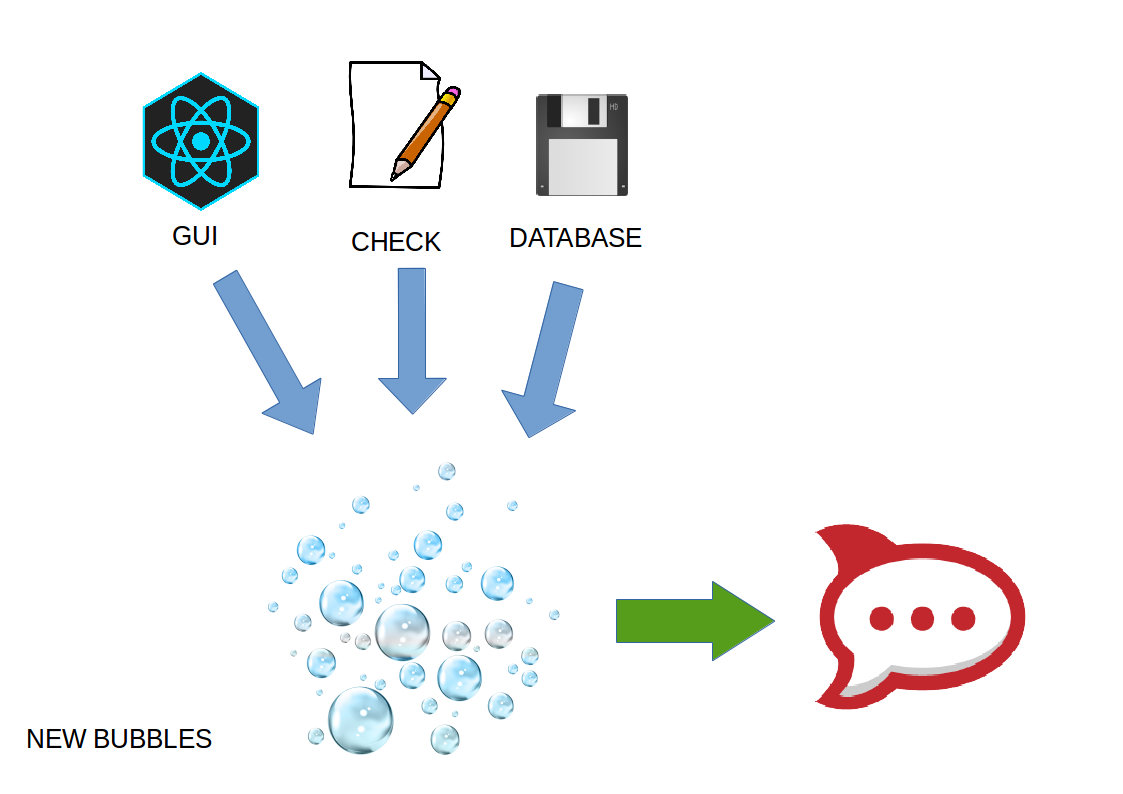
\includegraphics[width=\linewidth,height=.8\textheight,keepaspectratio]{img/uso_sdk.png}
  \end{center}
\end{frame}

\begin{frame}
  \begin{columns}[T] % align columns
    \begin{column}{.48\textwidth}
      \textbf{Creazione GUI}
      \begin{itemize}
      \item Bubble
        \begin{itemize}
        \item Sender
        \item Receiver
        \end{itemize}
        \pause
      \item Configuration Menu
      \item Button
        \begin{itemize}\pause
        \item[$ \rightarrow $] Personalizzazione
        \end{itemize}
      \end{itemize}
    \end{column}
    \pause
    \begin{column}{.48\textwidth}
      \textbf{Server Side Operations}
      \begin{itemize}
      \item[] Meteor.method
        \begin{itemize}
        \item insert  $ \rightarrow $ Custom method
        \item update $ \rightarrow $ Custom method
        \item remove
        \end{itemize}
      \end{itemize}
    \end{column}

  \end{columns}

\end{frame}
